\documentclass[compress]{beamer}
\usepackage{config_beamer} 

\title{Chapter 1: Univariate Analysis}
\subtitle{Introduction to Quantitative Methods}
\author{Maxime Chabriel}
\date{2024}

\begin{document}

\maketitle

\begin{frame}{Introduction}
    \begin{itemize}
        \item \textbf{Univariate analysis :} When we study only one variable \\
        \vspace{0.2cm}
        \item Distribution : How the values of a variable on multiple observations are spread
        \vspace{0.2cm}
        \item This chapter will be about understanding what is a distribution and how to simplify / study it 
        \vspace{0.2cm}
		\item Can you survive this class without understanding what is a distribution?
		\begin{itemize}
			\item Yes
			\item But if you do understand, everything else becomes easy to learn
		\end{itemize}
    \end{itemize}
\end{frame}

\section{Representing a distribution}
\begin{frame}[plain]
    \centering \Large
    \textbf{Representing a distribution} \\
	(NB this is by all means not an exhaustive list) \\
	\vspace{0.2cm}
	\begin{figure}
		\centering
		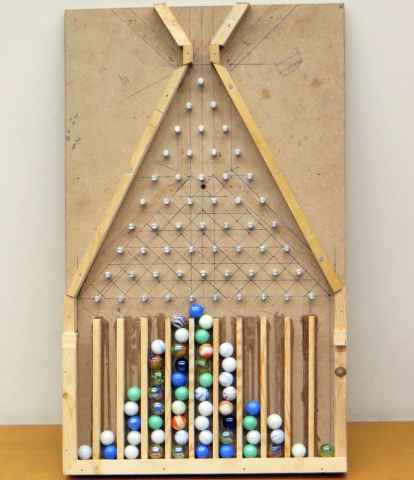
\includegraphics[scale=0.8]{Picture/Galton_Board_5.jpeg}
	\end{figure}
	\textit{A Galton board}
\end{frame}

\begin{frame}
	\textbf{Categorical / Discrete variables}
	\begin{itemize}
		\item The pie chart (circular graph, camembert). Good to represent proportions
		\begin{figure}
            \centering
            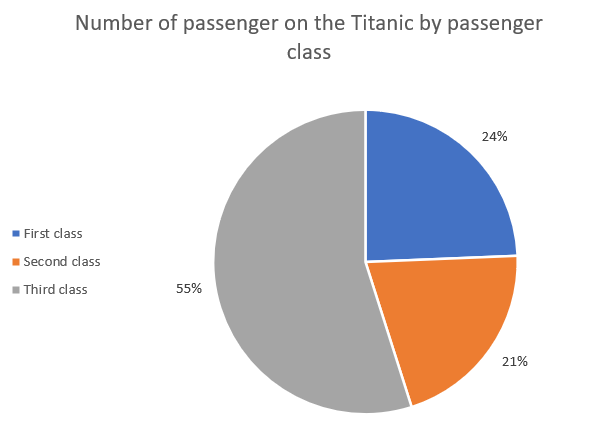
\includegraphics[scale=0.6]{Picture/Titanic pie chart.PNG}
        \end{figure}
	\end{itemize}
\end{frame}

\begin{frame}
	\textbf{Categorical / Discrete variables}
	\begin{itemize}
		\item The bar chart
		\begin{figure}
            \centering
            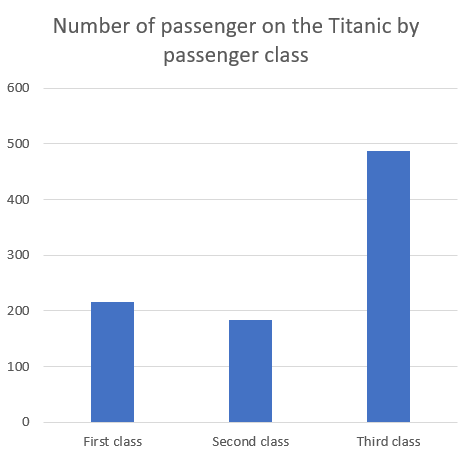
\includegraphics[scale=0.6]{Picture/Titanic bar chart.PNG}
        \end{figure}
	\end{itemize}
\end{frame}

\begin{frame}
	\textbf{Categorical / Discrete variables}
	\begin{itemize}
		\item The bar chart. Good to represent ordinal categorical variables or categorical variables with many modalities 
		\begin{figure}
            \centering
            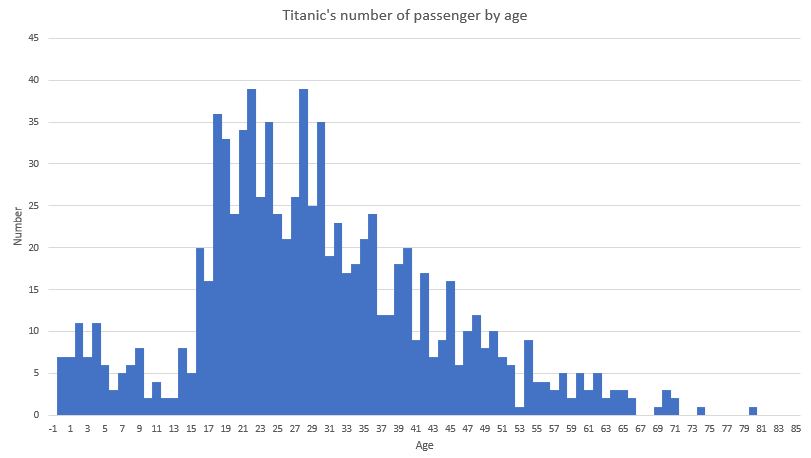
\includegraphics[scale=0.5]{Picture/Titanic bar chart passenger age.PNG}
        \end{figure}
		\item An age pyramid: https://www.insee.fr/fr/outil-interactif/5014911/pyramide.htm#!y=1991&v=2&l=en&c=0
	\end{itemize}
\end{frame}

\begin{frame}
	\textbf{Continuous values}
    \begin{itemize}
		\item Bar charts work fine on continous variables too (we then call them histograms). You just need to create some intervals (connoisseurs call them bins)
        \vspace{0.2cm}
        \begin{figure}
            \centering
            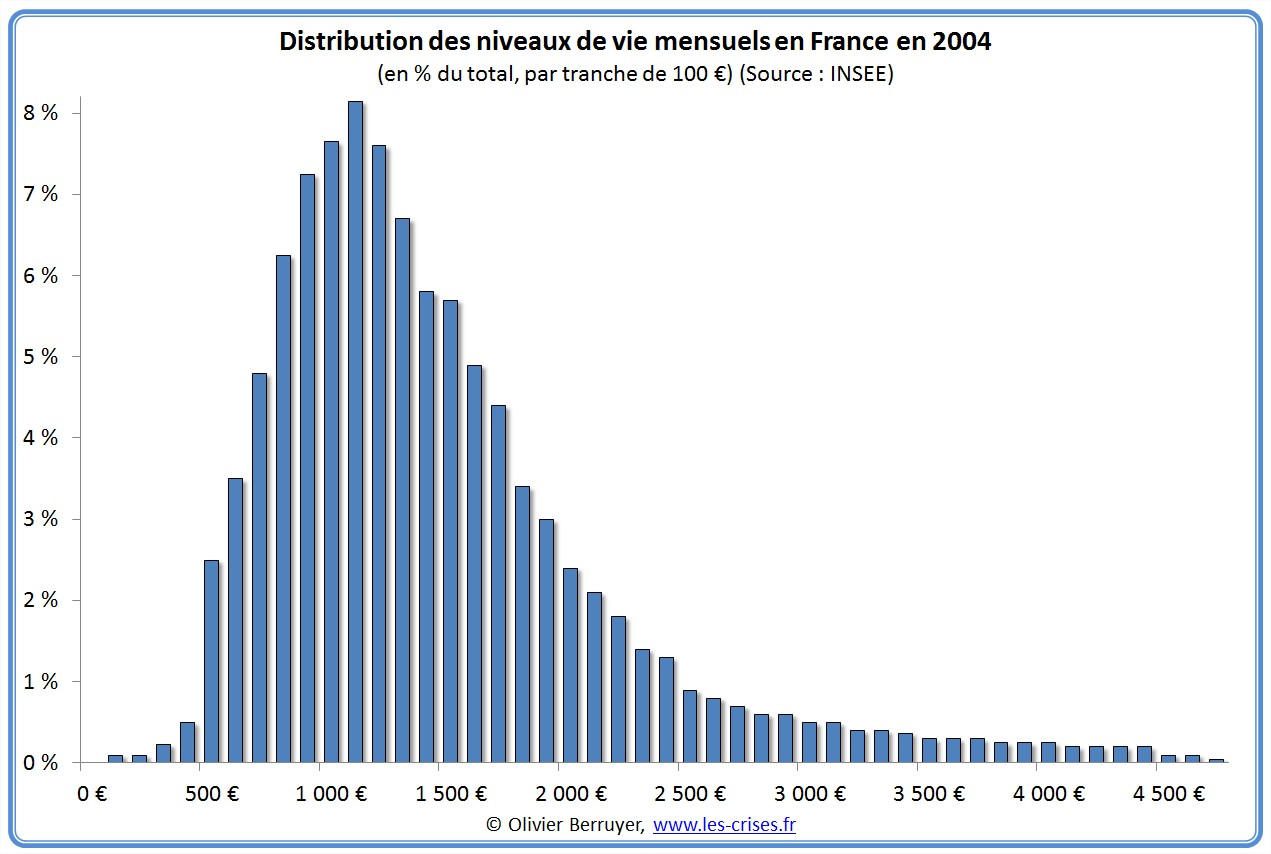
\includegraphics[scale=0.15]{Picture/distribution-niveaux-de-vie-mensuels.jpg}
        \end{figure}
    \end{itemize}
\end{frame}

\begin{frame}
	\begin{itemize}
		\item But otherwise, in practice we use a \textbf{density}
	\end{itemize}
	\begin{figure}
		\centering
		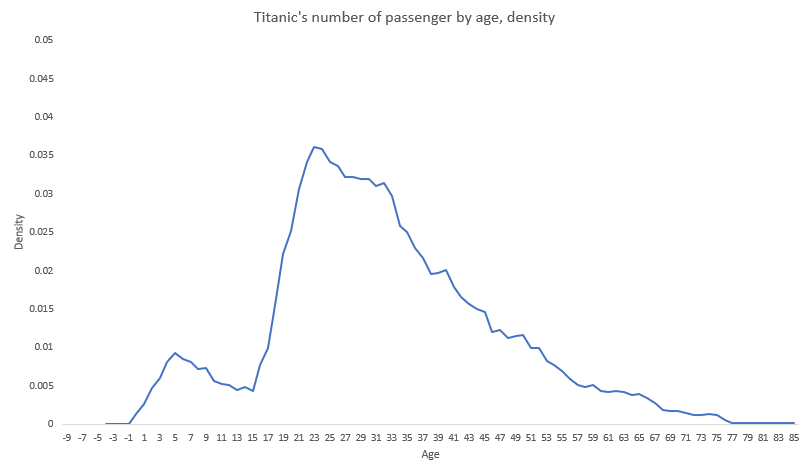
\includegraphics[scale=0.6]{Picture/Titanic age density.PNG}
	\end{figure}
\end{frame}

\begin{frame}
	\begin{itemize}
		\item How it is built (intuitive answer): We start from histogram bars
	\end{itemize}
	\begin{figure}
		\centering
		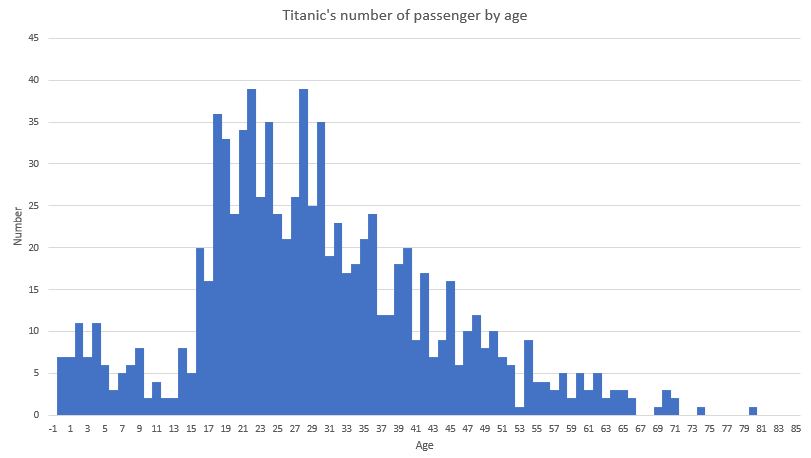
\includegraphics[scale=0.6]{Picture/Titanic bar chart passenger age.PNG}
	\end{figure}
\end{frame}

\begin{frame}
	\begin{itemize}
		\item How it is built (intuitive answer): We link the datapoints to create a line plot
	\end{itemize}
	\begin{figure}
		\centering
		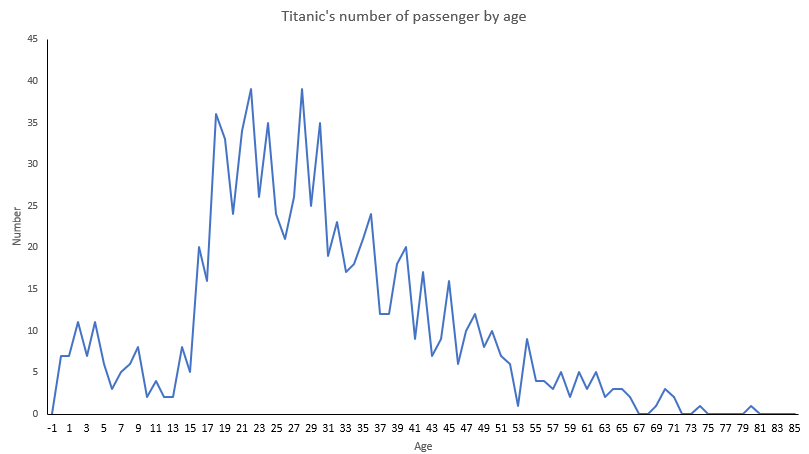
\includegraphics[scale=0.6]{Picture/Curve age titanic.PNG}
	\end{figure}
\end{frame}

\begin{frame}
	\begin{itemize}
		\item How it is built (intuitive answer): We smooth the line plot
	\end{itemize}
	\begin{figure}
		\centering
		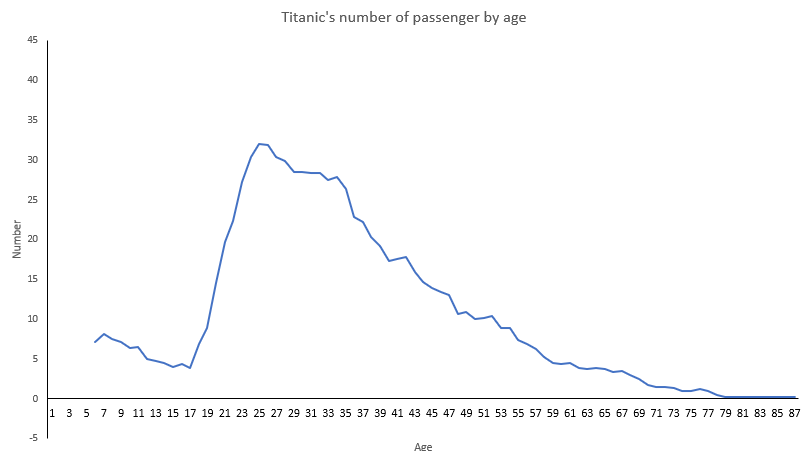
\includegraphics[scale=0.6]{Picture/Curve age titanic smoothed.PNG}
	\end{figure}
\end{frame}

\begin{frame}
	\begin{itemize}
		\item How it is built (intuitive answer): We rescale the y axis and stretch the plot so that is begins and ends by 0
	\end{itemize}
	\begin{figure}
		\centering
		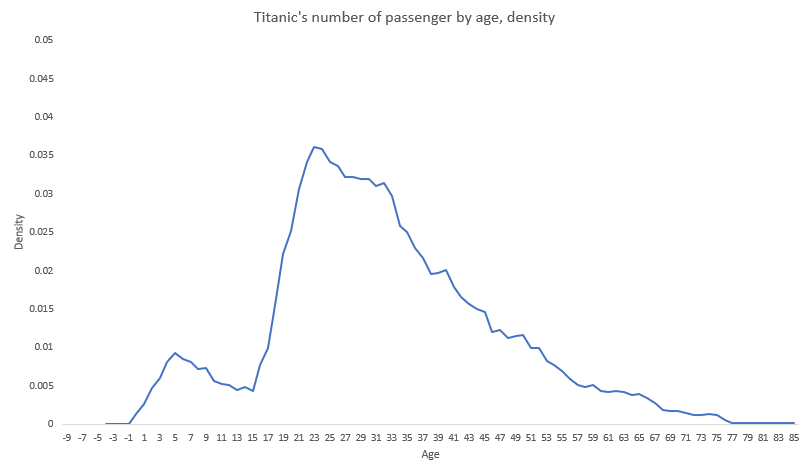
\includegraphics[scale=0.6]{Picture/Titanic age density.PNG}
	\end{figure}
\end{frame}

\begin{frame}
	\begin{itemize}
		\item But otherwise we use a \textbf{density plot}
		\vspace{0.2cm}
		\item How it is built (easy answer): smooth interpolation of the rescaled histogram bars
		\begin{itemize}
			\item Afik you cannot implement a density on Excel. We will do it in R in the final classes
			\item NB There are many algorithms out there to build a density, you do not need to know any. But you need to know how to read one
		\end{itemize}
		\item How to read it:
		\begin{itemize}
			\item A bit like a histogram (although the y axis is not directly readable)
			\item The area between a point $a$ and $b$ on the x axis represents the \% of the observations that are greater than $a$ and smaller than $b$
		\end{itemize}
	\end{itemize}
\end{frame}

\begin{frame}
	Example with the gaussian / normal density:
	\vspace{0.2cm}
	\begin{itemize}
		\item This density is very famous because it follows a lot of mathematical properties
		\begin{itemize}
			\item It is symetric
			\item It has infinite but thin tails
		\end{itemize}
		\vspace{0.2cm}
		\item And it is frequently found in nature!
		\begin{itemize}
			\item The height of people of similar age and sex
			\item The measurement error of the weight of a supermarket pasta bag
			\item By how much you miss when you play darts
			\item The random movements of atoms, particles, fluids...
			\item Some financial identicators (or are they?)
			\item etc.
		\end{itemize}
	\end{itemize}
\end{frame}

\begin{frame}
	\begin{figure}
		\centering
		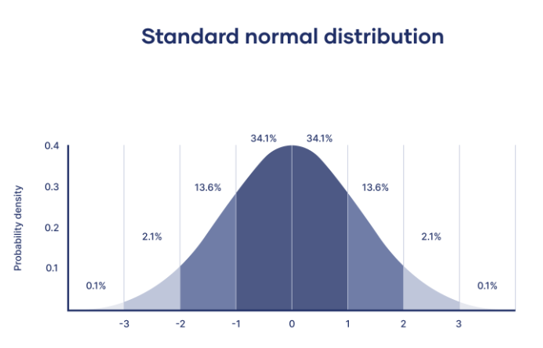
\includegraphics[scale=0.8]{Picture/exemple normal density.PNG}
	\end{figure}
\end{frame}

\begin{frame}
	\begin{figure}
		\centering
		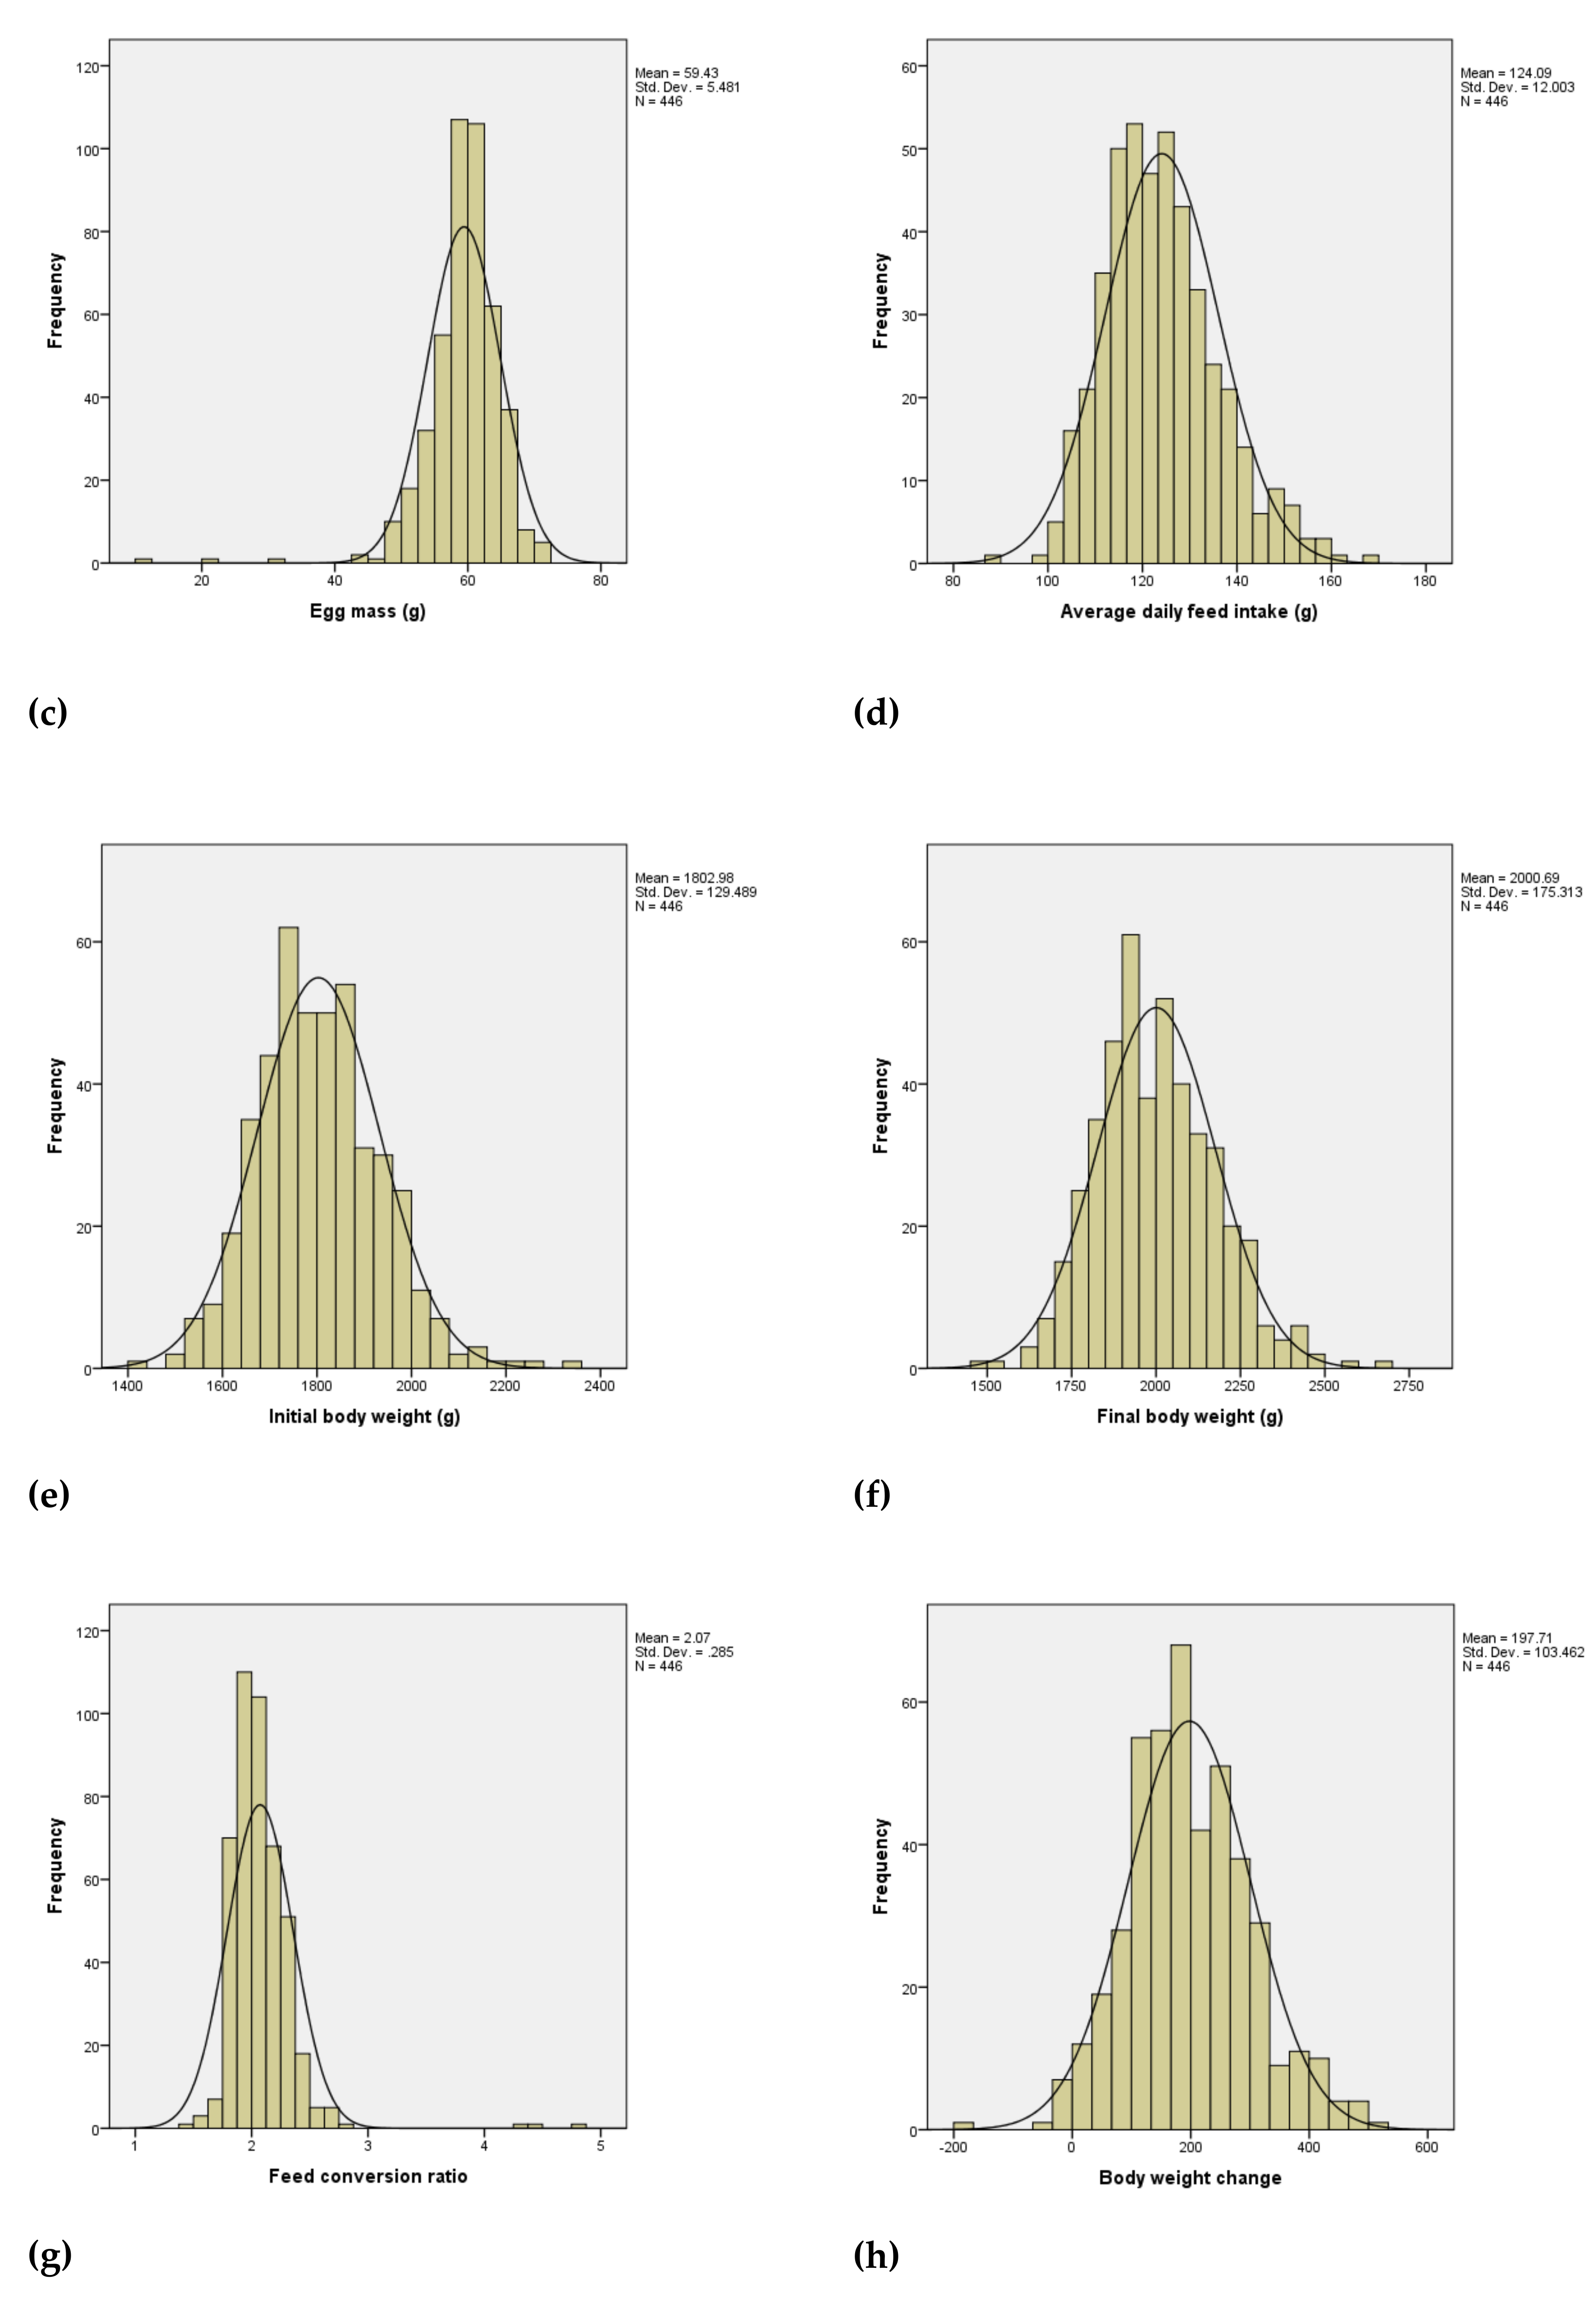
\includegraphics[scale=0.05]{Picture/hen eggs.png}
	\end{figure}
\end{frame}

\begin{frame}
	\begin{figure}
		\centering
		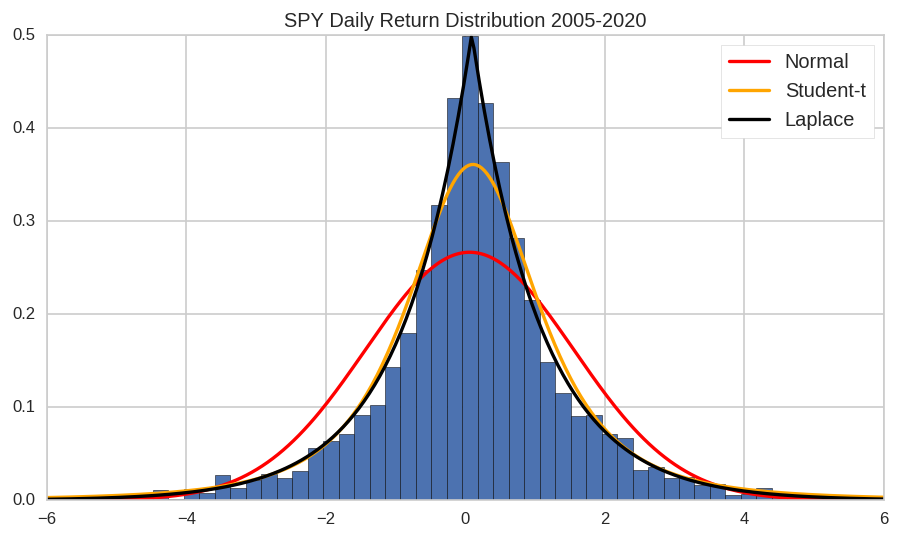
\includegraphics[scale=0.6]{Picture/SPY returns.png}
	\end{figure}
\end{frame}

\section{Statistics}
\begin{frame}[plain]
    \centering \Large
    \textbf{Statistics} \\
	(Congrats for making it this far, now the interesting stuff)
\end{frame}

\begin{frame}
	\begin{itemize}
		\item a \textbf{statistic}: A value built from a distribution. A good statistic gives interesting information on the distribution. Everything below \textit{are} statistics...
		\vspace{0.2cm}
		\item \textbf{maximum/minimum}
		\vspace{0.2cm}
		\item \textbf{mean}: What you would get if you shared all the values equally betwen each observation
	\end{itemize}
	\vspace{0.2cm}
	$E(X) = \sum_{i=1}^{N}\frac{X_{i}}{N}$ \\
	\vspace{0.2cm}
	\textit{X is the distribution of N values and $X_{i}$ is the ith value of X. The mean is equal to the sum of the values of the distribution divided by the number of values in the distribution}
	\vspace{0.2cm}
	\begin{itemize}
		\item \textbf{median}: The value greater than or equal to 50\% of the values of the distribution \textit{and} the value smaller than or equal to 50\% of the values of the distribution. When there are competing choices, we take the average of these choices
	\end{itemize}
\end{frame}

\begin{frame}
	\begin{figure}
		\centering
		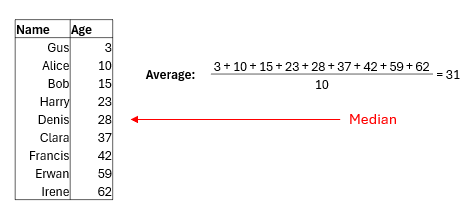
\includegraphics[scale=1]{Picture/Example mean median.PNG}
	\end{figure}
\end{frame}

\begin{frame}
	\begin{figure}
		\centering
		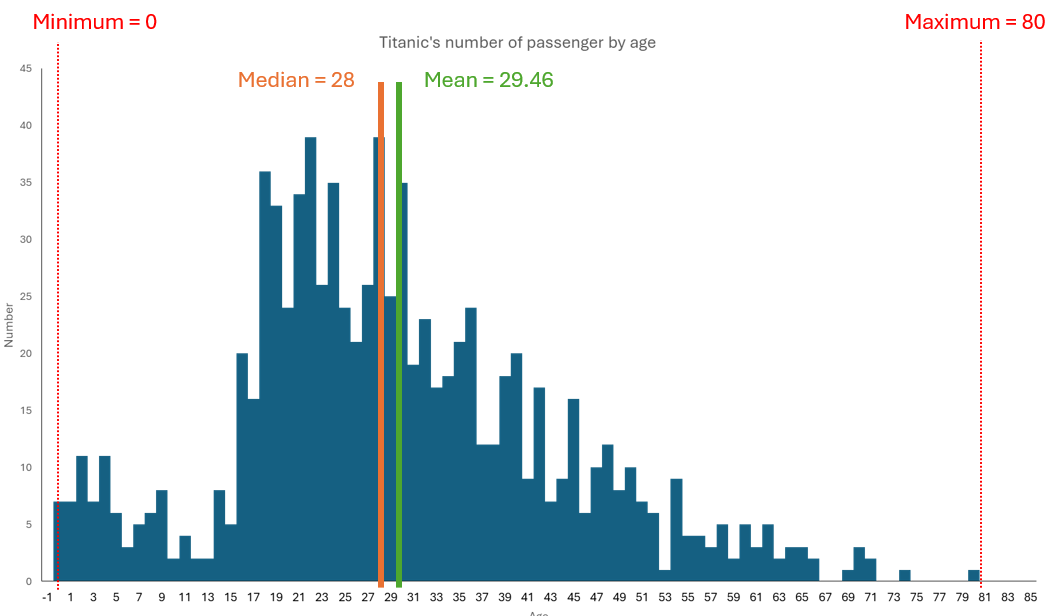
\includegraphics[scale=0.5]{Picture/Exemple titanic medium mediane.PNG}
	\end{figure}
\end{frame}

\begin{frame}
	\begin{itemize}
		\item \textbf{mode(s)}: Where the density gets its highest value. For discrete variables, this is the most frequent value in a distribution. NB There can be several modes
		\vspace{0.2cm}
		\item \textbf{quantiles}: Values that divide a distribution in equal groups
		\begin{itemize}
			\item Example: The median divides the distribution into 2 equal groups. The median \textit{is} a quantile
			\item Other types of quantiles: quartiles (divide in 4), quintiles (in 5), deciles (in 10), centiles (in 100)...
			\item \textit{median = 2nd quartile = 5th decile = 50th centile !}
		\end{itemize}
		\vspace{0.2cm}
		\item \textbf{variance}: How much the values of a distribution are spread out
		\begin{itemize}
			\item You might also encounter the \textbf{standard deviation}. This statistic can be \textit{very approximately} understood as the average distance between any value and the distribution's mean
		\end{itemize}
		\vspace{0.2cm}
		$V(X) = \sum_{i=1}^{N}(X_{i} - E(X))^{2}$ \\
		\vspace{0.2cm}
		$V(X) = \sigma(X)^2$
		\vspace{0.2cm}
	\end{itemize}
\end{frame}

\begin{frame}
	Example on Excel
\end{frame}

\begin{frame}
	\begin{figure}
		\centering
		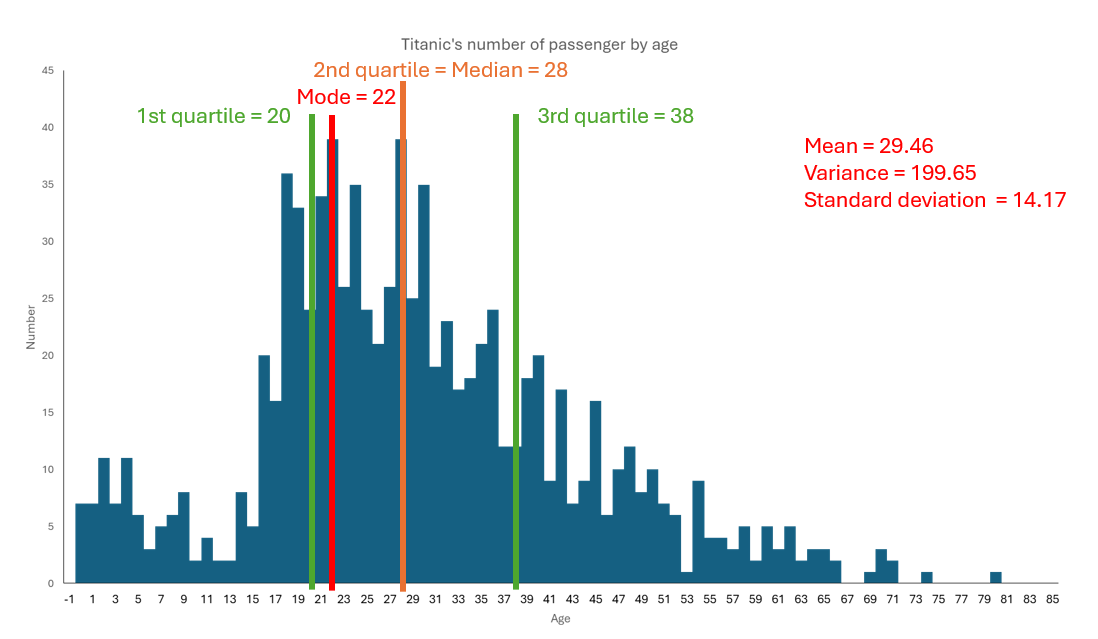
\includegraphics[scale=0.5]{Picture/Exemple titanic quartile.PNG}
	\end{figure}
\end{frame}

\begin{frame}
	\begin{itemize}
		\item \textbf{Outlier}: Values abnormally high or low. There is no absolute criterion to define an outlier. You can set them aside in your analysis \textbf{if and only if} you justify it properly and \textbf{always} say it when you do. You are that close from being the new Lysenko or Didier Raoult. Examples of what you are allowed to do:
		\vspace{0.2cm}
		\begin{itemize}
			\item The outliers exist because of an error in your data. Someone cheated at all his final exams and got better grades than everyone else
			\vspace{0.2cm}
			\item The outliers exist because your observations are not comparable. If you study sociodemographic values of some countries, you may set aside microstates
			\vspace{0.2cm}
			\item The outliers exist because of a random event. You compare currency trends and one country in your dataset is experiencing hyperinflation
		\end{itemize}
	\end{itemize}
\end{frame}

\begin{frame}
	\begin{itemize}
		\item But beware if:
		\vspace{0.2cm}
		\begin{itemize}
			\item The outliers are throwing off the scales of your graphs but they are important to your analysis. You study wealth distribution in a country and there are a few billionaires in your dataset
			\vspace{0.2cm}
			\item Some softwares/algorithms might automatically detect outliers using probabilistic criteria (units of standard deviation). These will always be mere suggestions, you make the final say!
			\vspace{0.2cm}
			\item When in doubt, don't
		\end{itemize}
	\end{itemize}
\end{frame}

\begin{frame}
	All the main statistics can be condensed into a \textbf{boxplot} (aka whisker plot, boîte à moustache):
	\begin{figure}
		\centering
		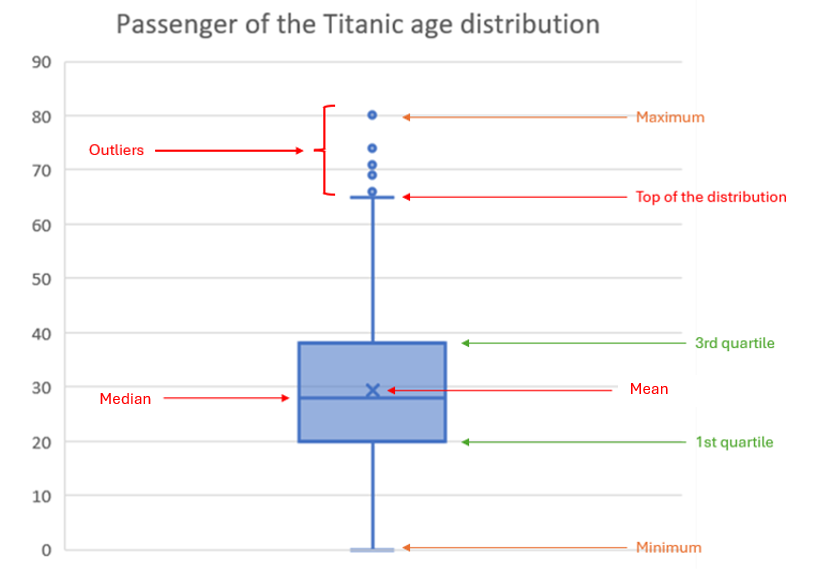
\includegraphics[scale=0.5]{Picture/boxplot.PNG}
	\end{figure}
\end{frame}

\begin{frame}
	Variations of the boxplot do exist. The only limit is your imagination! "Violin plots" done in R:
	\begin{figure}
		\centering
		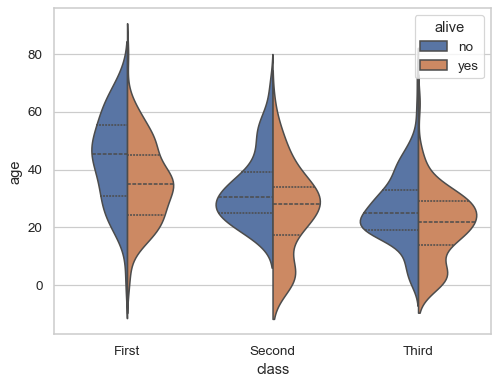
\includegraphics[scale=0.6]{Picture/violin titanic.png}
	\end{figure}
\end{frame}

\section{Choosing a statistic}
\begin{frame}[plain]
    \centering \Large
    \textbf{Choosing a statistic}
\end{frame}

\begin{frame}
	In practice, what is the difference between the mean and the median? Why do their values differ?
\end{frame}

\begin{frame}
	In practice, what is the difference between the mean and the median? Why do their values differ?
	\vspace{0.2cm}
	\begin{itemize}
		\item The mean is sensible to extreme (very high or very low) values
		\item The median is not very useful when there is a lot of dispersion
		\item If the mean is greater than the median, there are some extreme upper values. We say that the distribution is \textit{right-skewed}
		\item When someone only shows a mean, a median, or any other statistic, ask yourself, what about the rest of the data?
	\end{itemize}
\end{frame}

\begin{frame}
	Evolution of available income in French households (INSEE, euro 2018):
	\begin{figure}
		\centering
		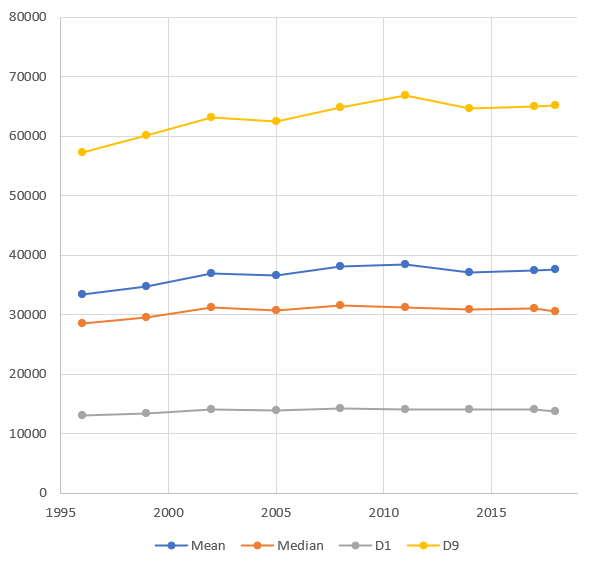
\includegraphics[scale=0.65]{Picture/french household income.PNG}
	\end{figure}
\end{frame}

\begin{frame}
	\begin{figure}
		\centering
		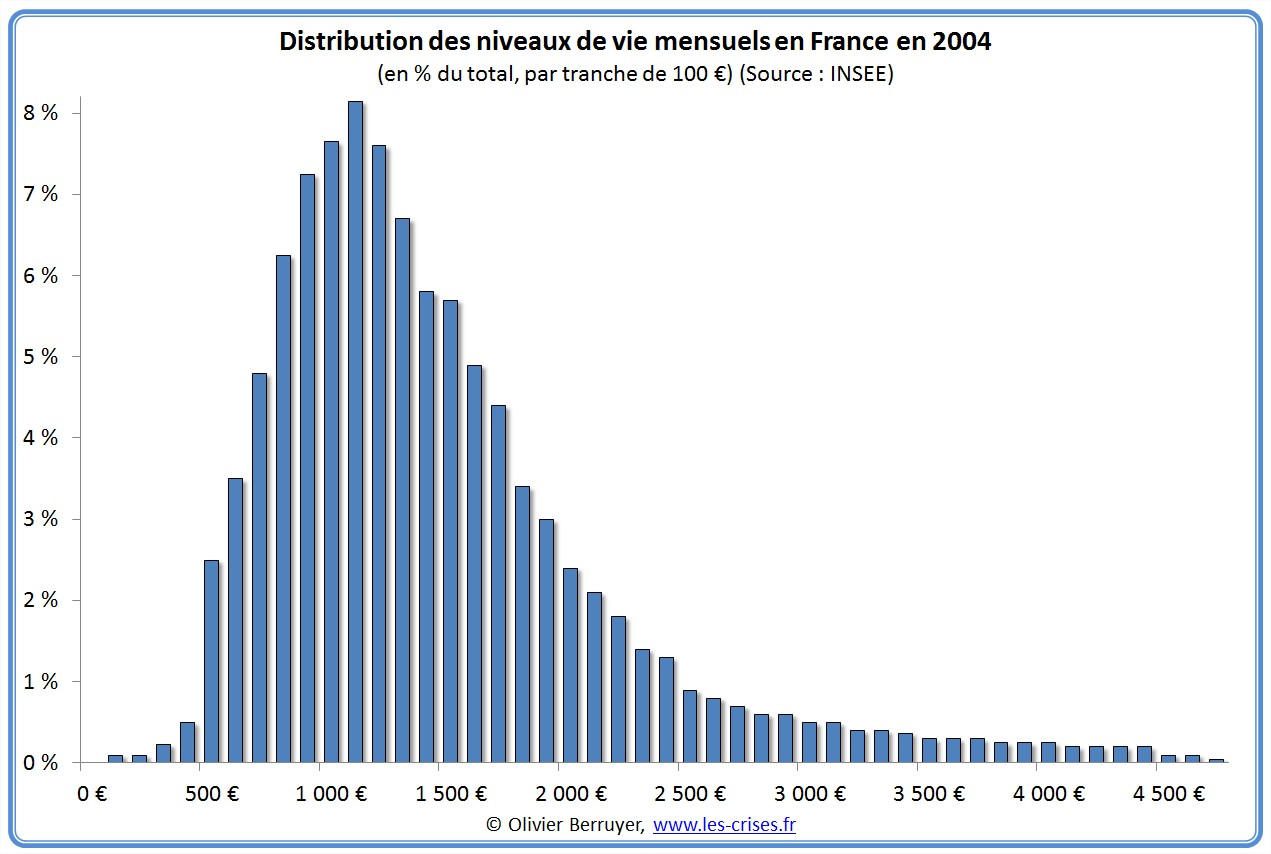
\includegraphics[scale=0.2]{Picture/distribution-niveaux-de-vie-mensuels.jpg}
	\end{figure}
\end{frame}

\begin{frame}
	Other famous statistics/inequality metrics:
	\vspace{0.2cm}
	\begin{itemize}
		\item \textbf{Gini coefficient}: Only for positive values (income for instance). 0 represents perfect equality (all the values of the distribution are the same). 1 means that all values except one equal 0 (1 observation has 100\% of the wealth)
		\vspace{0.2cm}
		\item \textbf{Interdecile ratio}: D9 divided by D1. How many times the 90th percentile is bigger than the 10th percentile
		\vspace{0.2cm}
		\item \textbf{Herfindhal index}: To measure how much a sum (a cake) is being divided. Mostly used in market competition analysis. 0 means that there are infinite values with equal shares (atomistic competition). 1 means there is only 1 observation with 100\% of the share (there is a monopoly)
	\end{itemize}
\end{frame}

\begin{frame}
	So how to choose a good statistic?
	\vspace{0.2cm}
	\begin{itemize}
		\item It depends on what you want to show. Or which measure has the most striking value (whether you like it or not, statistics are politics)
		\vspace{0.2cm}
		\item You do not need to choose only one. The more you include statistics in your analysis, the more your analysis will be convincing. Nuance is important!
		\vspace{0.2cm}
		\item Some measures are easier to understand than others. Think about your audience. Ex: Variance vs Interdecile ratio
	\end{itemize}
\end{frame}

\section{Comparing the distribution of variables}
\begin{frame}[plain]
    \centering \Large
    \textbf{Comparing the distribution of variables}
\end{frame}

\begin{frame}
	Some statistics can be directly used to compare variables:
	\vspace{0.2cm}
	\begin{itemize}
		\item Gini index
		\item Interdecile ratio
	\end{itemize}
	\vspace{0.2cm}
	Most are not, because they are \textbf{scale dependent}:
	\vspace{0.2cm}
	\begin{itemize}
		\item Mean, median
		\item Variance
	\end{itemize}
	\vspace{0.2cm}
	These are statistics that, if you changed the unit of the variable (km to m, € to \$, min to s...), they would change value! For these, you need to put the variables you compare in \textbf{the same unit}.
\end{frame}

\begin{frame}
	Depending on the context, you may also want to answer these questions:
	\vspace{0.2cm}
	\begin{itemize}
		\item Is the distribution \textbf{symetric}?
		\vspace{0.2cm}
		\item The \textbf{tails} of the distribution. Do they exist? Are they fat?
		\vspace{0.2cm}
		\item The \textbf{skewness}. Are the values more concentrated on the right (left skew)? Or the left (right skew)?
		\item Does the distribution looks like a \textbf{normal} (gaussian) distribution?
	\end{itemize}
\end{frame}

\begin{frame}
	\begin{figure}
		\centering
		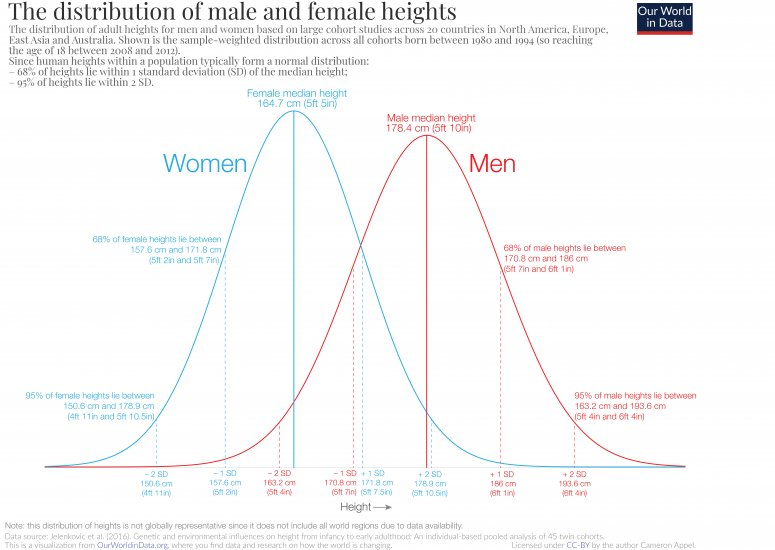
\includegraphics[scale=0.3]{Picture/men women height.jpeg}
	\end{figure}
\end{frame}

\begin{frame}
	Finally (reminder from the introduction), \textbf{always} ask yourself:
	\vspace{0.2cm}
	\begin{itemize}
		\item Are there some missing values? 
		\vspace{0.2cm}
		\item Is my sample representative of the population I am studying? 
		\vspace{0.2cm}
		\item Always question the quality / source of your data
	\end{itemize}
\end{frame}

\begin{frame}
	Your turn, practice time
\end{frame}

\end{document}